%------------------------------------------------------------------------------
% Stijl,Imports en Commando's
%------------------------------------------------------------------------------

%---------- Stijl ----------------------------------------------------
\documentclass{hogent-article}

%---------- Custom Commando's ----------------------------------------------------
\newcommand{\boldit}[1]{\emph{\textbf{#1}}} 
\newcommand{\customref}[1]{\underline{\ref{#1}: \nameref{#1}}}

%---------- Package imports ----------------------------------------------------
\usepackage{lipsum} % Voor vultekst
\graphicspath{{./grafieken/}}
\usepackage{subcaption}
\usepackage{float}

%------------------------------------------------------------------------------
% Metadata over het artikel
%------------------------------------------------------------------------------

%---------- Titel & auteur ----------------------------------------------------

% TODO: geef werktitel van je eigen voorstel op
\PaperTitle{Retrieval practice}
% TODO: geef op welk soort artikel dit is
% Dit is typisch de opdracht en het vak waarvoor dit artikel geschreven is, bv.
% ``Verslag onderzoeksproject Onderzoekstechnieken 2018-2019''
\PaperType{Verslag Onderzoek Onderzoekstechnieken 2018-2019}

% TODO: vul je eigen naam in als auteur, geef ook je emailadres mee!
\Authors{Wannes {De Craene}\textsuperscript{1},Michiel Schoofs\textsuperscript{2}, Lieven {Van Loo}\textsuperscript{3}, Wannes Sergeant\textsuperscript{4}}% Authors

% TODO: vul de naam van je co-promotor in.
% Als het hier gaat om een voorstel voor de bachelorproef, dan ben je hier
% verplicht de naam van je co-promotor in te vullen. Zoniet, dan kan je het
% leeg laten.
% Contactinfo: Geef hier de contactgegevens van elke auteur van het artikel (en
% indien van toepassing ook van de co-promotor).
\affiliation{
	\textsuperscript{1} \href{mailto:wannes.decraene.y0550@student.hogent.be}{mailto:wannes.decraene.y0550@student.hogent.be}
}
\affiliation{
	\textsuperscript{2} \href{mailto:michiel.schoofs@student.hogent.be}{mailto:michiel.schoofs@student.hogent.be}
}
\affiliation{
	\textsuperscript{3} \href{mailto:lieven.vanloo@student.hogent.be}{mailto:lieven.vanloo@student.hogent.be}
}
\affiliation{
    \textsuperscript{4} \href{mailto:wannes.sergeant@student.hogent.be}{mailto:wannes.sergeant@student.hogent.be}
}

\CoPromotor{}

%---------- Abstract ----------------------------------------------------------

\Abstract{Veel studenten hebben baat bij een betere studiemethode. De werkdruk in het onderwijs leidt tot stressvolle situaties; een betere methodiek kan helpen om de werkdruk te verlagen en de studenten een hoger slaagpercentage te geven. Met dit onderzoek proberen we een duidelijk overzicht te geven van de zogenaamde \boldit{Retrieval practice} methode. We bekijken de effecten van Retrieval practice voor groepen met een \boldit{Hoge} en \boldit{lage geheugencapaciteit}. Ook proberen we het type van memorisatie met deze techniek in kaart te brengen zijnde: \boldit{Rote} of \boldit{Memorisation}. Door middel van empirisch onderzoek proberen we eerdere studies te staven en verifiëren. We verwachten dat de conclusies van het eerder onderzoek correct zijn. Dat zou suggereren dat studenten met een lage geheugencapaciteit meer baat hebben bij Retrieval practice, en dat Retrieval practice tot Rote memorisatie leidt en geschikt om voor grote hoeveelheden uit het hoofd te leren, maar minder toepasselijk is bij leerstof waar effectief diepgaand begrip van de stof wordt verwacht.
}

%---------- Onderzoeksdomein en sleutelwoorden --------------------------------
% TODO: Vul de sleutelwoorden aan.


\Keywords{Onderzoekstechnieken; Retrieval Practice; Rote; Meaningful; Geheugencapaciteit}
\newcommand{\keywordname}{Sleutelwoorden}

%---------- Titel, inhoud -----------------------------------------------------

\begin{document}

\flushbottom % Makes all text pages the same height
\maketitle % Print the title and abstract box
\tableofcontents % Print the contents section
\thispagestyle{empty} % Removes page numbering from the first page

%------------------------------------------------------------------------------
% Hoofdtekst
%------------------------------------------------------------------------------

\section{Inleiding}

Retrieval practice en het zogenaamde test effect is door verschillende instellingen en experten al onderzocht, geprezen en genuanceerd. Zelfs tijdens het schrijven van deze literatuurstudie is er nieuw onderzoek verschenen door \textcite{Moreira_2019}. Door de hoeveelheid van studies en publicaties is het moeilijk om door de bomen het bos te zien. We zullen proberen aan de hand van een aantal onderzoeken een overzicht te geven van wat deze studiemethode inhoudt en hoe studenten het best kunnen gebruik maken van die studietechniek.\\
\par
\noindent
Concreet zullen we drie verschillende onderzoeken samenbrengen tot één experiment:\\
\begin{itemize}

\item Ons eerste doel is de originele studie van \textcite{Roediger_2006}  reproduceren en evalueren. We kijken met andere woorden of er inderdaad sprake is van het zogenaamde '\boldit{Test effect}'. - Voor meer informatie zie \customref{RetrievalPractice} -\\

\item Vervolgens willen we de studie van \textcite{Agarwal_2016} opnemen binnen ons onderzoek. Die studie suggereert dat mensen met een lagere geheugencapaciteit meer baat hebben bij Retrieval practice. - Zie ook\\ \customref{geheugencapaciteit} -\\

\item Tot slot bestuderen we nog het type van memorisatie dat bereikt wordt met Retrieval practice. Concreet onderscheiden we twee types van memorisatie, namelijk: ROTE en meaningful learning. Zoals het onderzoek van \textcite{van_Gog_2012} suggereert, verwachten we dat de studenten de informatie uit het hoofd leren (ROTE) zonder die effectief te begrijpen (Memorisation). -Zie ook \customref{RoteVSMeaningful} -
\end{itemize}

\section{Overzicht literatuur}

Voor we van start kunnen gaan met het onderzoek, moeten we eerst een literatuurstudie schrijven om duidelijk uit te lijnen welke bevindingen er al zijn binnen dit vakgebied. Die sectie dient eveneens voor het verduidelijken van de terminologie die we gebruiken binnen ons experiment. Na het lezen van de literatuurstudie hopen we dat de relevantie van de door ons gekozen variabelen duidelijk is.

\subsection{Retrieval Practice}
\label{RetrievalPractice}
Wat verstaan we nu juist onder de term `Retrieval Practice`? Concreet is dat een systeem waarbij je leerstof opneemt door het afnemen van testen, in de plaats van gewoon een boek te nemen en de leerstof op de conventionele manier in te studeren.\\
\par
\noindent
Om dat te verduidelijken halen we de methodiek aan zoals beschreven in het artikel van \textcite{Roediger_2006}. Een groep van testpersonen werd gevraagd om een nooit eerder geziene tekst uit het hoofd te leren volgens verschillende methodes.\\\\De eerste groep werd gevraagd om de tekst te bestuderen gedurende 20 minuten op de manier waarmee ze het meest vertrouwd waren. De andere groep kreeg slechts 5 minuten om de tekst te bestuderen en werd vervolgens gevraagd om gedurende 15 minuten de tekst te reproduceren op papier (het reproduceren op papier noemen we ook testen).\\

\par
\noindent
Die laatste methodiek, het bestuderen en vervolgens reproduceren op papier, duiden we aan als \boldit{Retrieval practice}. Uit de originele studie van Roediger en Karpicke bleek dat de groep die aan Retrieval practice deed veel meer van de originele tekst onthield na twee weken dan de groep die conventioneel studeerde. Dat fenomeen wordt aangeduid als het `\boldit{Testing effect}`.

\subsection{Onderscheid in geheugen capaciteit}
\label{geheugencapaciteit}
De studie van \textcite{Agarwal_2016} stelt dat er een onderscheid is tussen personen met een lage en hoge geheugencapaciteit. De bevindingen van het onderzoek wijzen uit dat Retrieval practice veel meer resultaat biedt bij proefpersonen met een lagere geheugencapaciteit. \textcite{Agarwal_2016} beweert zelfs dat Retrieval practice een effectieve leerstrategie kan zijn voor lager presterende studenten.\\
\par
\noindent
We zullen die studie reproduceren, door onze testgroep onder te verdelen in twee groepen. Voor een meer gedetailleerde uitleg zie \customref{methodologie}.

\subsection{Wat is leren?}
Wat wordt er nu exact verstaan onder de term '\textit{leren}'? Het artikel van \textcite{Mayer_2002} zegt dat leren niet enkel het verkrijgen van informatie is, maar ook het toepassen van die informatie op nieuwe en relevante situaties. Concreet definieert men in het artikel het leerproces in termen van twee fasen, namelijk:\\

\begin{itemize}
	\item \textbf{Het behouden van informatie}: hierbij zal de student de informatie bewaren over een lange periode van tijd. We spreken hier dus over het vermogen van de persoon om informatie te onthouden en die op te halen in haar originele vorm. We hebben het hier dus \underline{niet} over informatie interpreteren, maar puur over het memoriseren van de informatie zoals ze oorspronkelijk werd gepresenteerd.\\
	
	\item \textbf{Toepassen van informatie}: Hiermee bedoelt men het vermogen om de opgedane kennis toe te passen. Het  gaat hier dus niet alleen over het ophalen van informatie, maar eveneens het interpreteren en toepassen. Deze fase is dus een vervolg op de vorige fase en kan niet als losstaand beschouwd worden.
\end{itemize}

\subsection{Rote vs Meaningful Learning}
\label{RoteVSMeaningful}
Het artikel van \textcite{Mayer_2002} bestempelde die twee fasen eveneens als: Rote (Behouden van informatie) en Meaningful learning (Toepassen van informatie). Uit een vervolgstudie door \textcite{van_Gog_2012} blijkt dat Retrieval practice voornamelijk tot Rote-memorisatie leidt.\\

\par
\noindent
Met andere woorden is de proefpersoon door die techniek beter in staat de informatie op te halen in haar originele vorm. Indien men echter kijkt naar het vermogen van de persoon om die informatie te verwerken in concrete probleemsituaties, (\textit{Meaningful learning}) ziet men het omgekeerde effect. Men stelt in het onderzoek dat Retrieval practice zelfs nadelig is voor Meaningful learning en dat conventioneel studeren een betere optie is voor het verwerken van informatie.
\par
\noindent

\subsection{Retentie testen}
\label{RT}
Een ander begrip binnen Retrieval practice zijn de zogenaamde \boldit{retentietesten}. Een retentietest is een methode waarmee men gaat meten hoeveel informatie effectief onthouden is en die wordt gebruikt om de noodzakelijke data voor conclusies te verzamelen. In het originele experiment \textcite{Roediger_2006} werd gebruik gemaakt van een vragenlijst over de tekst.\\

\par
\noindent
Die methodiek kunnen we echter niet gebruiken als we het over Meaningful learning hebben, omdat die manier van testen voornamelijk dient om het behoud van informatie (Rote) te meten. Als reactie daarop ontwikkelde \textcite{Mayer_2002} een andere vorm van de retentietest. Het opzet van die ontwikkeling was om te bepalen hoe effectief de proefpersonen de aangereikte informatie hadden verwerkt.\\
\par
\noindent
Om de methode van Mayer het best weer te geven, maken we gebruik van zijn analogie. Hij stelde dat de gebruikte tekst over de wet van Ohm (een wet uit de natuurkunde) ging en de koppeling van die wet op elektrische circuits. Klassiek zou men vervolgens een vragenlijst geven over die wet en de aangereikte informatie. De methode die hij echter voorstelde was om zowel een reeks oefeningen op die wet te geven als een vraagstuk waarin de proefpersonen de wet moesten toepassen op een circuit en de resistentie bepalen. - Dat is ook de exacte methodiek die gebruikt werd in het onderzoek van \textcite{van_Gog_2012} om de mate van Meaningful learning te bepalen. -

\subsection{Invloed Feedback op Retrieval Practice}

Een belangrijke factor binnen het originele onderzoek van \textcite{Roediger_2006} was dat de zelftesten (na de originele studie van de tekst) zonder enige feedback waren. Dat wil zeggen dat indien de proefpersoon foutieve informatie opschreef op de zelftest, die informatie ook foutief werd opgenomen in het geheugen.\\
\par
\noindent
Uit het onderzoek van \textcite{Roediger_2011} leerden we dat feedback door externen zeker niet te verwaarlozen is. Het verschil tussen wel en geen feedback is aanzienlijk: in het geval van hun onderzoek waren de resultaten van de groep met feedback 30\% tot 64\% beter dan de testgroep zonder feedback.

\subsection{Invloed van voorkennis van de stof op de prestaties geleverd door Retrieval practice}
\label{voorkennis}
Een laatste stelling die we nog zouden willen meegeven is dat de mate van voorkennis geen invloed heeft op de resultaten geboekt met Retrieval practice.\\
\par
\noindent
Die stelling werd op de proef gesteld door het onderzoek van \textcite{Xiaofeng_2016}. In die studie onderzocht men het effect van voorkennis op twee verschillende studiemethodes, namelijk Elaboration en Retrieval practice. Elaboration is een techniek waarbij er gebruik gemaakt wordt van relaties tussen al bestaande kennis en nieuwe kennis, om op die manier efficiënter te leren. Uit dat onderzoek bleek dat bij Retrieval practice de mate van voorkennis weinig tot geen invloed had op de retention tests; in tegenstelling tot Elaboration.\\
\par
\noindent
Met andere woorden: studenten die al vertrouwd waren met het onderwerp van de gegeven tekst hadden geen voordeel ten opzichte van de groep die minder vertrouwd was met het onderwerp.

\section{Methodologie}
\label{methodologie}
Zoals al vermeld in de inleiding, en vervolgens uitgediept in de literatuurstudie, zijn er enkele factoren waar we zeker rekening mee willen houden in ons experiment. In deze sectie volgt een overzicht van de door ons gehanteerde methodes en werkwijzen. Daardoor kunnen we op een correcte en grondige manier conclusies trekken.

\subsection{Meten van geheugencapaciteit}
\label{methodology-gc}
Naar aanleiding van het artikel van \textcite{Agarwal_2016} gaan we onderzoeken of er een correlatie is tussen de geheugencapaciteit en de doeltreffendheid van Retrieval Practice. -Voor meer informatie zie ook sectie \\\customref{geheugencapaciteit}.- We moeten echter eerst verduidelijken hoe we die capaciteit meten in onze testgroepen.\\
\par
\noindent
We kunnen gebruik maken van een woordenlijst van 25 woorden, waarvan elk woord in lengte toeneemt. De proefpersoon in kwestie krijgt 5 minuten om de woordenlijst te memoriseren en wordt vervolgens gevraagd om die te reproduceren. Daarna wordt een score toegekend volgens het volgende principe: Een volledig correct geschreven woord krijgt 2 punten, een woord dat fonetisch correct is, krijgt 1 punt.\\
\par
\noindent
Met die methode zijn we in staat om de groep in twee delen op te splitsen. De groep die hoger scoorde dan de mediaan geven we het label \textit{Hoge geheugencapaciteit}, de overige groep  \textit{Lage geheugencapaciteit}

\subsection{Hervorming van de retentie test}
We gaan eveneens de retentietest veranderen. Dat doen we naar aanleiding van het artikel geschreven door \textcite{van_Gog_2012}. Concreet willen we het type van memorisatie (ROTE of Meaningful) door Retrieval Practice  bestuderen. -Voor meer informatie, zie sectie \customref{RT}.-\\
\par
\noindent
Aangezien het op dit moment nog niet duidelijk is welke tekst gebruikt gaat worden bij het experiment, kunnen we geen concrete retentietest opstellen. Graag geven we toch nog enkele opmerkingen mee die in acht genomen kunnen worden.\\
\par
\noindent
Om onze conclusies te kunnen staven, moeten we onderscheid maken tussen Rote en Meaningful learning. Dat heeft tot gevolg dat we twee types van retentietesten willen afnemen. Aan de ene kant willen we Rote learning meten. Dat kunnen we simpelweg bereiken met een vragenlijst waarbij de antwoorden regelrecht uit de aangereikte tekst komen. Aan de andere kant willen we Meaningful learning testen. Dat kunnen we doen aan de hand van de methode uitgelijnd in de publicatie van \textcite{Mayer_2002}. Concreet komt dat neer op het transformeren van de originele tekst naar oefeningen en vragen waarbij de informatie toegepast moet worden op ongeziene probleemstukken.

\section{Verwachte resultaten}

\subsection{Hypothesen}

\subsection{Duiding}

Analoog aan de artikels van \cite{HenryRoediger2006} en \cite{Agarwal2008}, zullen we gebruik maken van zowel grafieken als tabellen om onze hypotheses te staven. Op die manier kunnen we de gebruikte dataset vereenvoudigen en op een compacte en correcte manier conclusies trekken.\\
\par
\noindent
We zouden graag even stilstaan bij de verschillende variabelen en veronderstellingen die we gebruiken om de grafieken te maken. Zo hopen we foutieve communicatie te voorkomen.

\subsection{Grafieken}
\subsubsection{Uitleg}
De grafieken die we gebruiken zijn opgedeeld in twee groepen (uitgeleind in sectie \customref{methodology-gc}):
\begin{itemize}
	\item De groep met een \textit{lage geheugencapaciteit (LGC)}: dat is de testgroep die op de woordenlijsttest onder de mediaan scoorde. Die testgroep zit dus met andere woorden in de laagste 50\% van de afgenomen testen wat betreft hun score.
	\item De groep met een \textit{hoge geheugencapaciteit (HGC)}: dat is de groep die boven de mediaan scoorde. Kortom, de groep die bij de hoogste 50\% zit wat betreft hun score op de woordenlijst.
\end{itemize}
\subsubsection{Grafieken}
\begin{figure}[H]
	\begin{subfigure}{0.45\textwidth}
		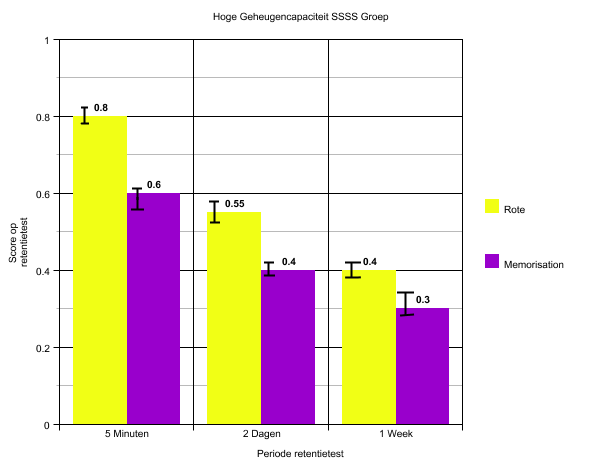
\includegraphics[width=\linewidth]{grafiek1}
		\caption{HGC Grafiek SSSS}
	\end{subfigure}
	\begin{subfigure}{0.45\textwidth}
		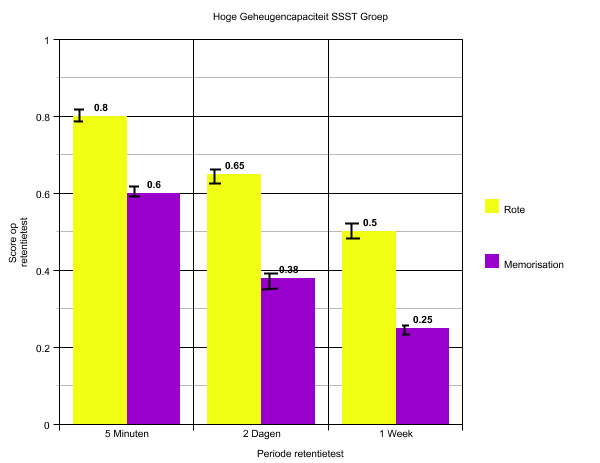
\includegraphics[width=\linewidth]{grafiek3}
		\caption{HGC Grafiek SSST}
	\end{subfigure}
	\begin{subfigure}{0.45\textwidth}
		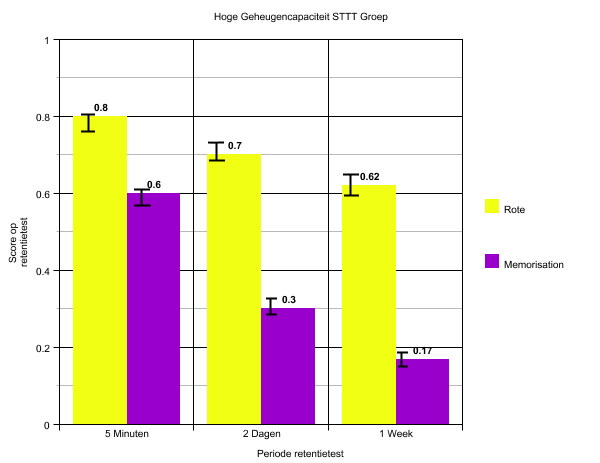
\includegraphics[width=\linewidth]{grafiek5}
		\caption{HGC Grafiek STTT}
	\end{subfigure}
	\caption{Grafieken van de Hoge Geheugencapaciteit groep}
\end{figure}
\begin{figure}[H]
    \begin{subfigure}{0.45\textwidth}
        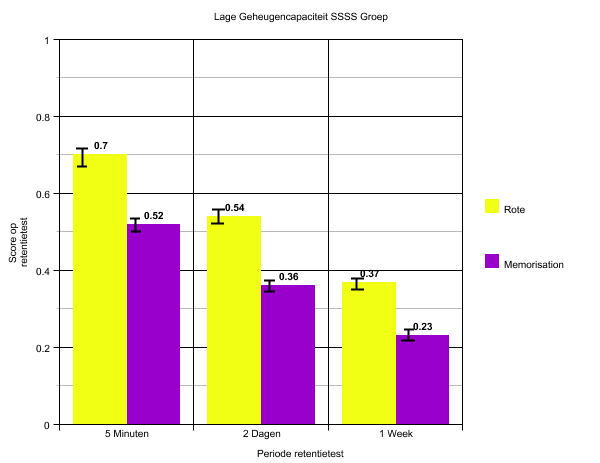
\includegraphics[width=\linewidth]{graph2}
        \caption{LGC Grafiek SSSS}
    \end{subfigure}
    \begin{subfigure}{0.45\textwidth}
        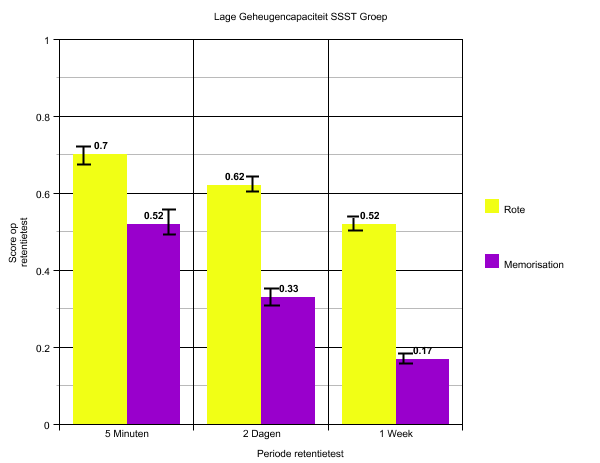
\includegraphics[width=\linewidth]{graph4}
        \caption{LGC Grafiek SSST}
    \end{subfigure}
    \begin{subfigure}{0.45\textwidth}
        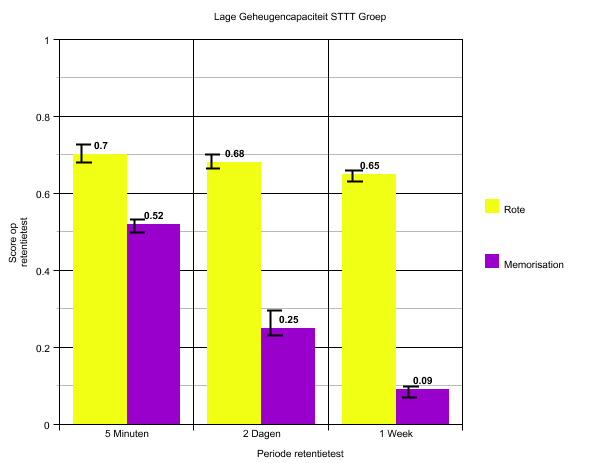
\includegraphics[width=\linewidth]{graph6}
        \caption{LGC Grafiek STTT}
    \end{subfigure}
    \caption{Grafieken van de Lage Geheugencapaciteit groep}
\end{figure}
\begin{figure}[H]
    \begin{subfigure}{0.45\textwidth}
        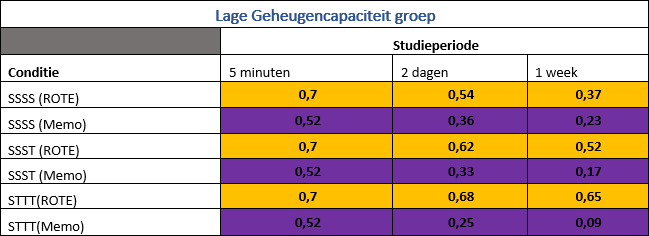
\includegraphics[width=\linewidth]{table1}
        \caption{LGC Grafiek SSSS TODO}
    \end{subfigure}
    \begin{subfigure}{0.45\textwidth}
        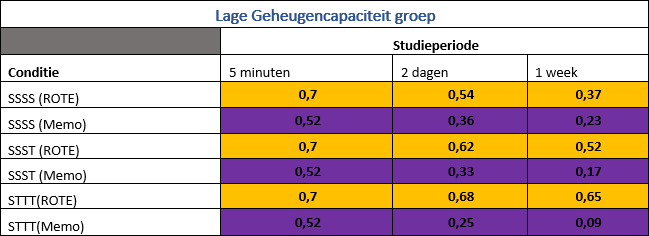
\includegraphics[width=\linewidth]{table2}
        \caption{LGC Grafiek SSST TODO}
    \end{subfigure}
    \caption{Grafieken van de Lage Geheugencapaciteit groep TODO}
\end{figure}
\section{Conclusie}

\subsection{Variabelen}
Concreet hebben wij beslist om een extra variabele te introduceren, namelijk de geheugencapaciteit van het proefpubliek. Ook hebben wij beslist om de retentietest te hervormen volgens twee principes: Rote en Meaningful Learning (lees: uit het hoofd leren en kunnen toepassen).\\
\par
\noindent    
Verder delen we de proefpersonen op in drie groepen, zoals in het originele experiment van \cite{Henry2006} , Die zijn: Study-Study-Study-Study, Study-Study-Study-Test  en Study-Test-Test-Test. 

\subsection{Hypothesen en resultaten}

\noindent
Eerst en vooral verwachten we gelijksoortige resultaten als die uit vooraf afgenomen onderzoek door \cite{Henry2006}. Dat wil zeggen dat mensen die aan Retrieval practice doen, beter zouden moeten scoren dan mensen die op de conventionele manier studeren.\\
\par
\noindent
Bovendien verwachten we ook dat mensen met een lage geheugencapaciteit iets meer vooruitgang zullen zien wanneer ze gebruik maken van Retrieval Practice.\\
\par
\noindent
Ten slotte verwachten we een beter resultaat bij de groepen studenten die aan Rote learning doen, in vergelijking met studenten die Meaningful learning toepassen.


\section{Addendum}

Verder hebben we nog enkele artikels die zeer nuttige informatie bevatten, maar die niet absoluut noodzakelijk zijn om het experiment succesvol af te werken.

\subsubsection{Successful inhibition, unsuccessful retrieval: Manipulating time and success during retrieval practice}

Hier wordt hetzelfde onderwerp behandeld, maar op een omgekeerde manier. In het vooraf uitgevoerde experiment van \cite{HenryRoediger2006} testte men op het behouden van informatie, terwijl \cite{BenjaminStorm2009} net analyseerde wat de proefpersonen vergaten. Dat is dus niet echt een noodzakelijk artikel, maar het is wel interessant om te zien dat het omgekeerde experiment tot zo goed als dezelfde resultaten leidt. 

\subsubsection{Commentary: Retrieval practice protects memory against acute stress}

\cite{Smith2016} bekijkt welke invloed ``Retrieval Practice'' heeft op stress. Hoewel dat wel een goede variabele zou zijn om op te nemen in dergelijke onderzoeken, hebben wij beslist om onze focus ergens anders te leggen.

\subsubsection{Optimizing retrieval as a learning event: When and why expanding retrieval practice enhances long-term retention}

Dit artikel, geschreven door \cite{Storm2010}, is zo goed als een ``kopie'' van het artikel van \cite{HenryRoediger2006}. Dat kunnen we dus ook niet echt opnemen in onze studie, maar het is handig om te zien dat een volledig losstaand onderzoek tot zeer gelijksoortige conclusies komt. 

\subsubsection{Retrieval Practice Produces More Learning than Elaborative Studying with Concept Mapping}

Aangezien men spreekt over een nieuwe studiemethode, was het ook interessant om te bekijken of er naast Retrieval Practice nog andere methodes zijn zijn die de retentie van geziene leerstof bevorderen. \cite{JeffreyKarpicke2011} voegt daar een extra studiemethode genaamd ``Concept Mapping'' aan toe. Dat was ook een leuke variabele geweest voor ons onderzoek, maar zoals voordien vermeld zijn wij een andere weg opgegaan.

%------------------------------------------------------------------------------
% Referentielijst
%------------------------------------------------------------------------------

\phantomsection
\printbibliography[heading=bibintoc]

\end{document}
